
\begin{frame}{Projective Metrics}{Motivation}
	\vspace{-1cm}
	\begin{itemize}
		\item Introduced by Gabidulin and Simonis (1997)\\~\\
		\item\uncover<2->{A \textbf{generalization} of many metrics in coding theory\\~\\}
		\item \uncover<3->{Related to (projective) \textbf{finite geometry}, \textbf{combinatorics}, \textbf{matroids}, \textbf{graph theory}, etc. \\~\\}
		
		\item \uncover<4->{\textbf{Sweet-spot} for research on metrics?\\~\\~\\}
	\end{itemize}

\uncover<7->{

\begin{center}
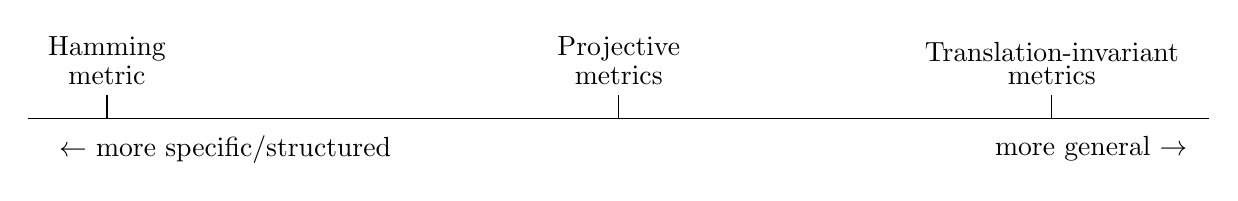
\begin{tikzpicture}

\uncover<5->{
\draw (1,0.6) node[above] {Hamming};
\draw (1,0)--(1,0.3) node[above] {metric};
\draw (7.5,0.6) node[above] {Projective};
\draw (7.5,0)--(7.5,0.3) node[above] {metrics};
\draw (13,0.6) node[above] {Translation-invariant};
\draw (13,0)--(13,0.3) node[above] {metrics};
}
\draw	
(0,0)--(15,0);

\draw (2.5,-0.1) node[below]  {$\leftarrow$	more specific/structured};
\draw (15-1.5,-0.1) node[below]  { more general $\rightarrow$};
\end{tikzpicture}
\end{center}
}

\end{frame}
 %but first, let me tell you how i got interested in this topic


 \begin{frame}{}{Projective metrics}
	
	Let $\cF = \{f_1,\ldots,f_N\} \subset V$ be a set of 
	such that $\langle f_1, f_2, \ldots, f_N \rangle = V$.\\~\\~\\

	\uncover<2->{
	The \textbf{projective weight function} $\wt_{\cF}(\cdot): V \to \mathbb{N}_{\geq 0}$ corresponding to  $\cF$ is 	
\[
\wt_{\cF}(x) := \min\{ t \in \mathbb{N}_{\geq 0} \,\,|\,\,  x \textnormal{ is in the linear span of } t \textnormal{ projective points } \langle f_i \rangle  \in \cF \}
\]
\text{}\\
}
\uncover<4->{
The \textbf{projective metric} $d_{\cF}(\cdot, \cdot): V \times V \to \mathbb{N}_{\geq 0}$ corresponding to $\cF$ is 	
\[
d_{\cF}(x,y) := \wt_{\cF}(y-x).
\]
}
\end{frame}





\begin{frame}{}{}
	\vspace{-1.5cm}
	Hamming metric
	\begin{equation*}
	\left(\begin{array}{c>{\columncolor{red!20}}ccc>{\columncolor{red!20}}cc>{\columncolor{red!20}}c}
	0  & 1  & 0 & 0 & 1 & 0 & 1\\
	\end{array}\right) \quad 	\uncover<2->{\to \; \cF = \{ \text{spans of standard basis vectors} \}}
	\end{equation*}
	
	\uncover<3->{
		Rank metric
		\begin{equation*}
		\left(\begin{array}{>{\columncolor{blue!20}}c>{\columncolor{blue!20}}c>{\columncolor{blue!20}}c}
		0  & 1  & 0 \\
		1  & 1  & 0 \\
		1  & 1  & 1 \\
		\end{array}\right)  \quad \uncover<4->{\to \; \cF = \{ \text{spans of rank 1 matrices} \}}
		\end{equation*}
	}
	
	\uncover<5->{
		Sum-Rank metric
		\begin{equation*}
		\left(\begin{array}{>{\columncolor{blue!20}}c>{\columncolor{blue!20}}c>{\columncolor{blue!20}}c|>{\columncolor{red!20}}c>{\columncolor{red!20}}c>{\columncolor{red!20}}c|>{\columncolor{green!20}}c>{\columncolor{green!20}}c>{\columncolor{green!20}}c}
		0  & 1  & 0 & 0  & 1  & 0 & 1  & 0  & 1 \\
		1  & 1  & 0 & 0  & 0  & 0 & 1  & 0  & 1 \\
		1  & 1  & 1 & 0  & 1  & 0 & 0  & 0  & 0 \\
		\end{array}\right)  \quad\uncover<6->{\to \; \cF = \left\{ \text{spans of } \big( \text{ some 0 blocks } \big| \text{ rank 1 matrix } \big| \text{ some 0 blocks }\big) \right\}}
		\end{equation*}
	}
	
	\uncover<7->{
		Cover metric (rows and columns)
		\begin{equation*}
		\left(\begin{array}{c>{\columncolor{red!20}}cccc}
		0  & 1  & 0 & 0 & 0\\
		\rowcolor{red!20}
		0  & 1  & 0 & 1 & 1\\
		0  & 1  & 0 & 0 & 0\\
		\rowcolor{red!20}
		1  & 0  & 0 & 1  & 0\\
		\end{array}\right)  \quad \uncover<8->{\to \; \cF = \left\{ \text{spans of matrices with 1  non-zero row or 1 non-zero column} \right\}}
		\end{equation*}
	}
	
	\uncover<9->{
		Phase-rotation metric
			\begin{equation*}
			\left(\begin{array}{cccc}
			1  & 1  & 0 & 1\\
			\end{array}\right) = \left(\begin{array}{cccc}
			\rowcolor{red!20}
			1  & 1  & 1 & 1\\
			\end{array}\right) + \left(\begin{array}{cc>{\columncolor{red!20}}cc}
			0  & 0 & 1 &  0\\
			\end{array}\right)  \quad  \uncover<10->{\to \; \cF = \left\{ \text{spans of standard basis vectors or all-1} \right\}}
			\end{equation*}
	
	}

	\text{}\\~\\\text{}
\end{frame}



\contourlength{1.0pt}

\begin{frame}{}{}
\vspace{-5cm}
%\only<1-2>{\uncover<2-2>{Strongly regular Clebsch graph / Greenwood–Gleason graph}}
\only<1-1>{Vertices: vectors of $\F_2^4$}
\only<2-4>{Distance from $0000$ to $1101$: \uncover<3->{\textcolor{red}{red:} 3,} \uncover<4->{\textcolor{blue}{blue:} 2}}
%\only<7->{\textbf{Phase-rotation metric:} an edge is a Hamming error or the \alert{all-bits-flip error}}
\only<5->{Graph distance on Clebsch graph  \,\,$=$\,\, \textbf{Phase-rotation metric/distance} on $\F_2^4$}\\
\uncover<6->{An edge is a Hamming error or the \alert{all-bits-flip error}}
\begin{center}
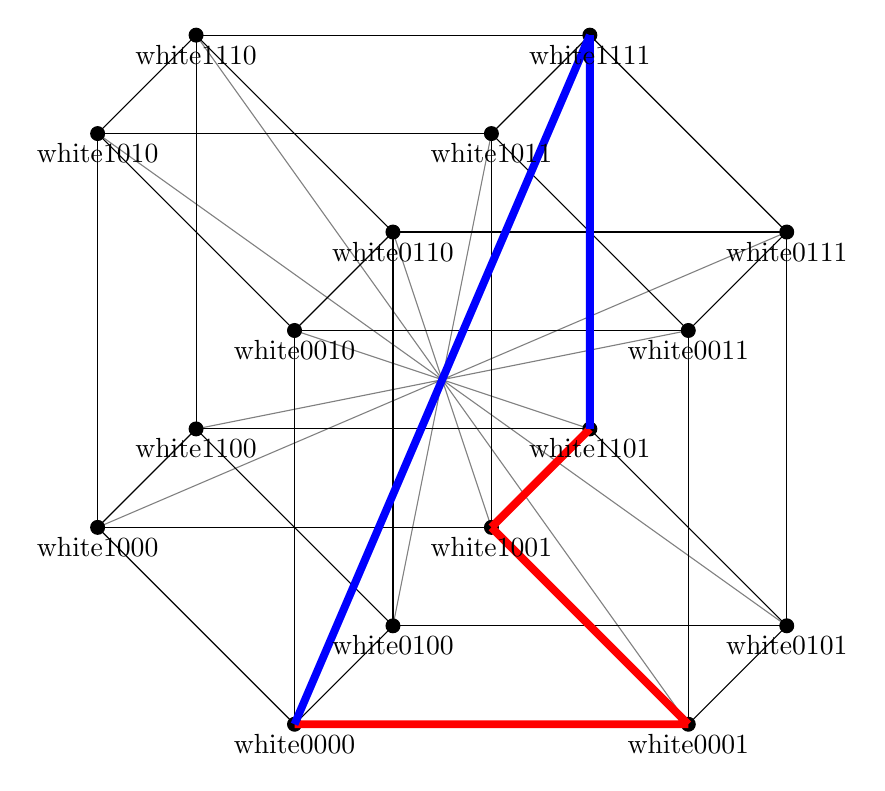
\begin{tikzpicture}[yscale=2.5, xscale=2.5, rotate=0]

\coordinate (0000) at (1,1);
\coordinate (0001) at (3,1);
\coordinate (0010) at (1,3);
\coordinate (0011) at (3,3);
\coordinate (0100) at (1.5,1.5);
\coordinate (0101) at (3.5,1.5);
\coordinate (0110) at (1.5,3.5);
\coordinate (0111) at (3.5,3.5);

\coordinate (1000) at (0,2);
\coordinate (1001) at (2,2);
\coordinate (1010) at (0,4);
\coordinate (1011) at (2,4);
\coordinate (1100) at (0.5,2.5);
\coordinate (1101) at (2.5,2.5);
\coordinate (1110) at (0.5,4.5);
\coordinate (1111) at (2.5,4.5);


\draw[gray]
(0000) -- (1111)
(0010) -- (1101)
(0100) -- (1011)
(0110) -- (1001)
(1000) -- (0111)
(1010) -- (0101)
(1100) -- (0011)
(1110) -- (0001)
;

\draw
(0000) -- (0001)
(0010) -- (0011)
(0100) -- (0101)
(0110) -- (0111)
(1000) -- (1001)
(1010) -- (1011)
(1100) -- (1101)
(1110) -- (1111)
;


\draw
(0000) -- (0010)
(0001) -- (0011)
(0100) -- (0110)
(0101) -- (0111)
(1000) -- (1010)
(1001) -- (1011)
(1100) -- (1110)
(1101) -- (1111)
;

\draw
(0000) -- (0100)
(0001) -- (0101)
(0010) -- (0110)
(0011) -- (0111)
(1000) -- (1100)
(1001) -- (1101)
(1010) -- (1110)
(1011) -- (1111)
;

\draw
(0000) -- (1000)
(0001) -- (1001)
(0010) -- (1010)
(0011) -- (1011)
(0100) -- (1100)
(0101) -- (1101)
(0110) -- (1110)
(0111) -- (1111)
;





\filldraw[black] (0000)  circle (1pt);
\filldraw[black] (0001)  circle (1pt);
\filldraw[black] (0010)  circle (1pt);
\filldraw[black] (0011)  circle (1pt);
\filldraw[black] (0100)  circle (1pt);
\filldraw[black] (0101)  circle (1pt);
\filldraw[black] (0110)  circle (1pt);
\filldraw[black] (0111)  circle (1pt);

\filldraw[black] (1000)  circle (1pt);
\filldraw[black] (1001)  circle (1pt);
\filldraw[black] (1010)  circle (1pt);
\filldraw[black] (1011)  circle (1pt);
\filldraw[black] (1100)  circle (1pt);
\filldraw[black] (1101)  circle (1pt);
\filldraw[black] (1110)  circle (1pt);
\filldraw[black] (1111)  circle (1pt);


\uncover<3->{
	\draw[line width=1.0mm, red]
	(0000) -- (0001)
	(0001) -- (1001)
	(1001) -- (1101)
	;}

\uncover<4->{
	\draw[line width=1.0mm, blue]
	(0000) -- (1111)
	(1111) -- (1101)
	;}


\uncover<1->{

\draw (0000) node[below] {\contour{white}{0000}};
\draw (0001) node[below] {\contour{white}{0001}};
\draw (0010) node[below] {\contour{white}{0010}};
\draw (0011) node[below] {\contour{white}{0011}};
\draw (0100) node[below] {\contour{white}{0100}};
\draw (0101) node[below] {\contour{white}{0101}};
\draw (0110) node[below] {\contour{white}{0110}};
\draw (0111) node[below] {\contour{white}{0111}};

\draw (1000) node[below] {\contour{white}{1000}};
\draw (1001) node[below] {\contour{white}{1001}};
\draw (1010) node[below] {\contour{white}{1010}};
\draw (1011) node[below] {\contour{white}{1011}};
\draw (1100) node[below] {\contour{white}{1100}};
\draw (1101) node[below] {\contour{white}{1101}};
\draw (1110) node[below] {\contour{white}{1110}};
\draw (1111) node[below] {\contour{white}{1111}};
}




\end{tikzpicture}
\end{center}

\vspace{-5cm}
%\vspace{-10cm}
%\uncover<1-2>{\text{}\hspace{13cm}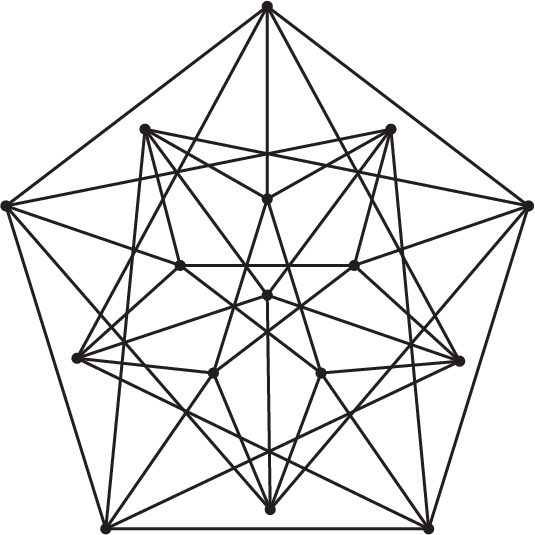
\includegraphics[scale=0.2]{clebsch3.png}}



\end{frame}


\begin{frame}{Equivalent notions - 2 }{Subspace Arrangments}
     For a set \(I \subset \cF\) let \(F_I \coloneqq \langle f \mid f \in I\rangle \). 
    For \(t \in \bN\) consider the subspace arrangement \( \mathcal{A} \coloneqq \{F_I \mid dim(F_I) = t\}\). Then we have \(B_t(0) = \cup_{F_I \in \cA}F_I\). By exclusion/inclusion we have 
    \begin{equation}
        |B_t(0)| = \sum_{J \subset \cA} (-1)^{|J|+1}|\cap_{F \in J}F|
    \end{equation}
    An other version is obtained by considering the lattice: \(\cL_{\cA} \{\cap_{F \in J}F | J \subset \cA\}\) ordered by reverse inclusion.
    \begin{equation}
        |\bF^n_q \setminus B_t(0)|= \sum_{x \in \cL_{\cA}}\mu(\bF_q^n,x) card(x)
    \end{equation}
    Where \( \mu\) is the Möbius function of \(\cL_{\cA}\).

\end{frame}

\begin{frame}{Equivalent notions - 2 }{Subspace Arrangments}
\begin{itemize}
	\item For some subspace arrangements the  Möbius function of some subspace arrangements is known.
	\item It may be useful to try to understand whether any of these can be induced by a projective metric. 
	\item This also points in the direction of trying to study the homology group of the lattice associated to a sphere of a projective metric.
	\item Ideas on how this might work are very welcome! :)
\end{itemize}
\end{frame}

\begin{frame}{Equivalent notions - 3}{Known Hamming codes}
	A very important connection to Classical Coding theory is given by the following.
	\begin{definition}(Parent functions and Parent codes of $\cF$)
		The \myfont{parent functions} of $\cF$ are $\Ff_q$-linear functions $\varphi: \Ff_q^{\N} \to V$ such that $\langle \varphi( e_i ) \rangle = F_{\sigma(i)} \in \cF$ for some $\sigma(i) \in S_{\N}$.
		The \myfont{parent codes} of $\cF\subset \Gr_1(V)$ are the elements in the class $\bar \C := [\ker (\varphi)]$ where \([\ker (\varphi)]\) is the equivalence class of $\ker(\varphi)$ and \(\varphi\) is a parent function of $\cF$.
	\end{definition}

Given \(v \in \cV\) the parent code \(\cC\) describes all the possible linear combinations of \(\cF\) that equal to \(v\).
That is we have: \(v = \sum_{f \in \cF} a_ff = \sum_{f \in \cF} b_ff \) that is \(v = \varphi(a) = \varphi(b)\) if and only if \( a-b \in \cC\). 
A series of important proprieties depends on this code, for example we have that:
% \begin{observation}
% \end{observation}
If \(x \in \mathbb{F}_q^\mathbb{N}\) satisfies \(\wt_H(x) \leq \frac{d_H(\mathcal{C})}{2}\), then \(\wt_H(x) = \wt_\mathcal{F}(\varphi(x))\).


\end{frame}


\begin{frame}{}{}
	\vspace{-1cm}
	
	Equivalent notions of $\wt_{\cF}(\cdot)$ in different contexts:\\~\\
	
	
	\begin{itemize}
	\item \uncover<2->{\textbf{Graph theory:}\\ Cayley graph of $\F_q^n$ with generating set $\cF$; $\,\,$ } \uncover<3->{ $\wt_{\cF}(v) $ is graph distance between $v$ and $0$. \\~\\}
	
	\item \uncover<4->{\textbf{Coding theory:}\\
		Certain code $\C$ (depends on $\cF$); } \uncover<5->{ $\,\,$  $\wt_{\cF}(v)$ is  Hamming weight of the coset $(v+\C)$.\\~\\}
	
	\item \uncover<6->{\textbf{Projective geometry:} \\
		Flats spanned by points in $\cF$; $\,\,$} \uncover<7->{ $\wt_{\cF}(v) $ is smallest rank of such a flat that contains $v$.\\~\\}
	
	\item \uncover<8->{\textbf{Subspace arrangments}
		A ball of size \(t\) in projective metric corresponds to the size of the \textbf{subspace arrangement} generated by subsets of \(\cF\) of size less than \(t\).
                
		}
		
		\uncover<10->{\textbf{Q:} General ways to calculate $\wt_{\cF}(v)$?\\}
		\uncover<11->{\textbf{Q:} For fixed $t$, how many $v$ have $\wt_{\cF}(v) = t$? \(\rightarrow \)  Hamming like bound. }
		
		\uncover<12->{\item Please let me know if you know a (partial) answer in any of these contexts! :)\\~\\}
		
	\end{itemize}
\end{frame}







\begin{frame}{}{What can we do?}
\vspace{-1.5cm}
\uncover<2->{Singleton-type bound!\\~\\}

\uncover<3->{Let $V$ be an $n$-dim vector space over $\F_q$. Let $\cF$ be a spanning family for a projective metric.\\}
\uncover<4->{
\begin{definition*}
	\textnormal{
	Let $t \in \{0,1,2,\ldots,n\}$. We define $\mu_{\cF}(t)$ as the maximum cardinality of a subset $\cG \subseteq \cF$ satisfying
	\begin{enumerate}
		\item \uncover<5->{All $f_i \in \cG$ are linear independent from each other over $\F_q$;}
		\item \uncover<6->{All $v \in \langle \cG \rangle$ have $\wt_{\cF}(v) \leq t$.}
	\end{enumerate}
}
\end{definition*}
}

\uncover<7->{
\begin{theorem}[\textbf{General Singleton-type bound}] 

 \scalebox{1.1}{Let $\C \subseteq V$ be a subset and let $d = \min\{d_{\cF}(x,y) \,|\, x \neq y \in \C)\}$. Then}
	\[
	\scalebox{1.2}{$|\C| \leq q^{n - \mu_{\cF}(d-1)} \leq q^{n-d+1}$
}
	\]
\end{theorem}
}

\uncover<8->{
	\textbf{Coincides} with Singleton bounds for specific projective metrics!
}
\end{frame}

\begin{frame}{Characterization of projective metrics }{What can we do?}


Where two codes are equivalent if there exists a linear Hamming isometry sending one onto the other. The following result tells us that a projective metric is univocally determined by it's parent code.
\begin{theorem}
    
    Let $ \bar Pr_{\N}(V)$ be the set containing the equivalence classes of projective metrics on $V$ of size $\N$ and $\bar Gr_{\N-N}(\Ff_q^{\N})$ be the set containing the equivalence classes of subspaces of $\Ff^{\N}_q$ of dimension $\N - N$. Then there exists a bijection:
    \begin{align*}
    \Psi: \bar Pr_{\N}(V) &\to \bar Gr_{\N-N}(\Ff_q^{\N}) \\
    \bar w_{\cF} &\mapsto \bar \C_{\cF}
\end{align*}
    Where $\bar \C_{\cF}$ is the parent code of $\cF$.
\end{theorem}

\end{frame}
\begin{frame}{Characterization of projective isometries}{What can we do?}
    
\begin{definition}
    An \(\F\)-isometry is a linear isomorphism \(L:V \to V\) such that \(L(\cF) = \cF\). The set of \(\F\)-isometries, with the operation of composition, forms a group denoted as \(isom_{\F}(V)\).
\end{definition}

\begin{theorem}
Let \(stab_H(\C)\) be the stabilizer of the parent code \(\C\) respect to the Hamming isometries, then \(isom_{\cF}(V) \cong stab_H(\C)\)
\end{theorem}

% \begin{theorem}
%     \(isom_{\cF}(V) \cong stab_H(\C)\). The group isomorphism is given by \(\Psi: stab_H(\C) \to isom_{\cF}(V)\) where \(\Psi(F) = \hat F\), the unique \(\cF\)-isometry such that the following diagram commutes:
%     \[\begin{tikzcd}[ampersand replacement=\&]
%         V \arrow[r,"F"] \& V \\
%         \Ff_q^{\N} \arrow[u,"\varphi"] \arrow[r,"\hat F"'] \& \Ff_q^{\N} \arrow[u,"\varphi"']
%     \end{tikzcd}\]
% \end{theorem}
\end{frame}

\begin{frame}{Constructions}{What can we do?}
\vspace{-1cm}
\uncover<2->

\uncover<3->{
We can define
\[
\wt_{\cF} \cup \wt_{\cG} := \wt_{\cF \cup \cG}
\]
 and
\[
\wt_{\cF} \otimes \wt_{\cG} := \wt_{\cF \otimes \cG}
\]
where $\cF \otimes \cG := \{\langle f_i \rangle \otimes \langle g_i \rangle \,\,|\,\, \langle f_i \rangle \in \cF, \,\langle g_i \rangle \in \cG \}$\\~\\
}

\uncover<4->{
\textbf{Example}\\

Let $\cF = \{\text{all 1-dim subspaces of } V\}$. Then $\wt_{\cF}(x) = 1$ for all $x\neq 0$. This is the \textbf{discrete weight} $\wt_{\operatorname{Dis}}$.\\~\\
}

\uncover<5->{

\textbf{Examples}\\
\begin{itemize}
	\item \uncover<6->{
		\scalebox{1.2}{$\wt_{\operatorname{Dis}} \otimes \wt_{\operatorname{Dis}} = \wt_{\operatorname{Rank}}$} \\}%\,\,\,\, (on $V_1 \otimes V_2$)
	\item \uncover<7->{\scalebox{1.2}{$\wt_{\operatorname{H}} \otimes \wt_{\operatorname{Rank}} = \wt_{\operatorname{Sum-rank}}$}\\}
	\item\uncover<8->{ \scalebox{1.2}{$\wt_{\operatorname{Dis}} \otimes \wt_{\operatorname{H}} = \wt_{\operatorname{Row}}$}\\}
	\item \uncover<9->{\scalebox{1.2}{$\wt_{\operatorname{H}} \otimes \wt_{\operatorname{Dis}} = \wt_{\operatorname{Column}}$}\\}
	\item \uncover<10->{\scalebox{1.2}{$\wt_{\operatorname{Row}} \cup \wt_{\operatorname{Column}} = \wt_{\operatorname{Cover}}$}}
\end{itemize}

}
\end{frame}




\begin{frame}{}{Current research}
\vspace{-0.5cm}
\begin{itemize}
	\item Algorithms for calculating  $\wt_{\cF}(v)$ for $v \in V$
\item Are there general methods for obtaining sphere sizes $|\{v \in V \,|\, \wt_{\cF}(v)=t\}|$ for $t \in \mathbb{N}$?
\item Is there a natural way do generilize other concepts of coding theory? Dual Codes? Perfect Codes? ecc...
\item Approach?: using poset lattice of projective metrics, where $\wt_{\cF} \preccurlyeq \wt_{\cG} $ iff $\cF \subseteq \cG $
\end{itemize}


\begin{center}
	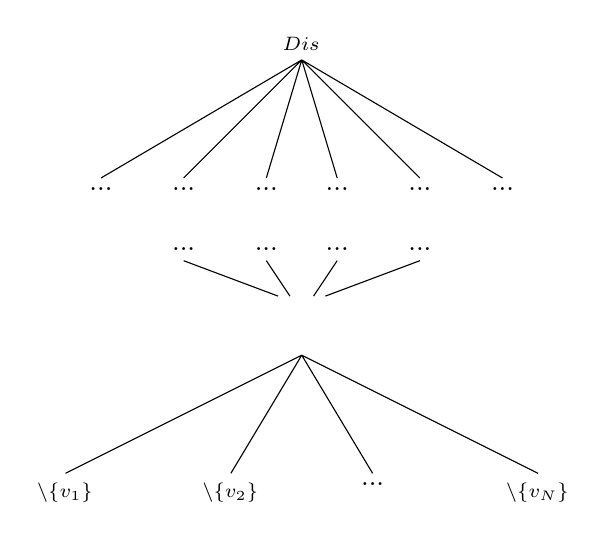
\begin{tikzpicture}[yscale=1.5, xscale=1.5, rotate=0]
	
	\draw (0,0) node[above] {$\wt_{\operatorname{Dis}}$}--(-1, -1) node[below] {...}
	(0,0) --(-0.3, -1) node[below] {...}
	(0,0) --(0.3, -1) node[below] {...}
	(0,0) --(1, -1) node[below] {...}
	(0,0) --(1.7, -1) node[below] {...}
	(0,0) --(-1.7, -1) node[below] {...}
	;
	
	
	\draw (0,-2.5) node[above] {$\wt_{\cF}$}--(-2, -3.5) node[below] {$\wt_{\cF \setminus \{v_1\}}$}
	(0,-2.5) --(-0.6, -3.5) node[below] {$\wt_{\cF \setminus \{v_2\}}$}
	(0,-2.5) --(0.6, -3.5) node[below] {...}
	(0,-2.5) --(2, -3.5) node[below] {$\wt_{\cF \setminus \{v_N\}}$}
	;
	
	\draw (-0.2,-2) -- (-1, -1.7) node[above] {...}
	(-0.1,-2) -- (-0.3, -1.7)  node[above] {...}
	(0.1,-2) -- (0.3, -1.7)  node[above] {...}
	(0.2,-2) -- (1, -1.7)  node[above] {...}
	;
	
\end{tikzpicture}
\end{center}



\end{frame}

